\section{Introduction}
This software is intended for use to calibrate, view, and analyze spectrum collected from various nuclear instrumentation. The document serves as the primary usage document. This software was developed using Python 3.8 and PyQt5 using packages such as Matplotlib and NumPy. The software has been developed into an executable file such that it can be run as any other program, this is done using PyInstaller. All code is considered open source. \\

This software is very much in beta phase testing, as such bugs and glitches are to be expeceted. You should report such bugs to the developer or care holder of the software upon discovery of such issues.

\section{Install and Initial Opening of Software}
This software is provided in a zip folder named Spectrum\_Viewer.zip, this folder contains all required libraries and packages for the software to run on a Windows configured machine. Before operation the software first must be unzipped, the built in method doing this in Windows10 should suffice. In the unzipped folder there will be 2 items, a folder named ``Spectrum\_Viewer'' and a shortcut `Spectrum''. The file contains all necessary files to launch the application, this files should not be moved. The shortcut is a shortcut to launch the application, this can be drag and dropped for ease of use. There is  a known bug when attempting to start the software from various biulds of Windows. If you experience these issues, you will either be forced to run the software from source or install serval packages and build the software against the specific build.\\

The interface will open a window containing three main areas, shown below in Figure \ref{fig:opening}. The left most window will be populated when spectrum are loaded. The right most window will be populated when spectrum are added to the graph. The center section features a full featured graphing utility. This graphing tool bar features the capabiltiy to zoom, pan, save, as well as other varius graphing features.

\begin{figure}[h!]
	\centering
	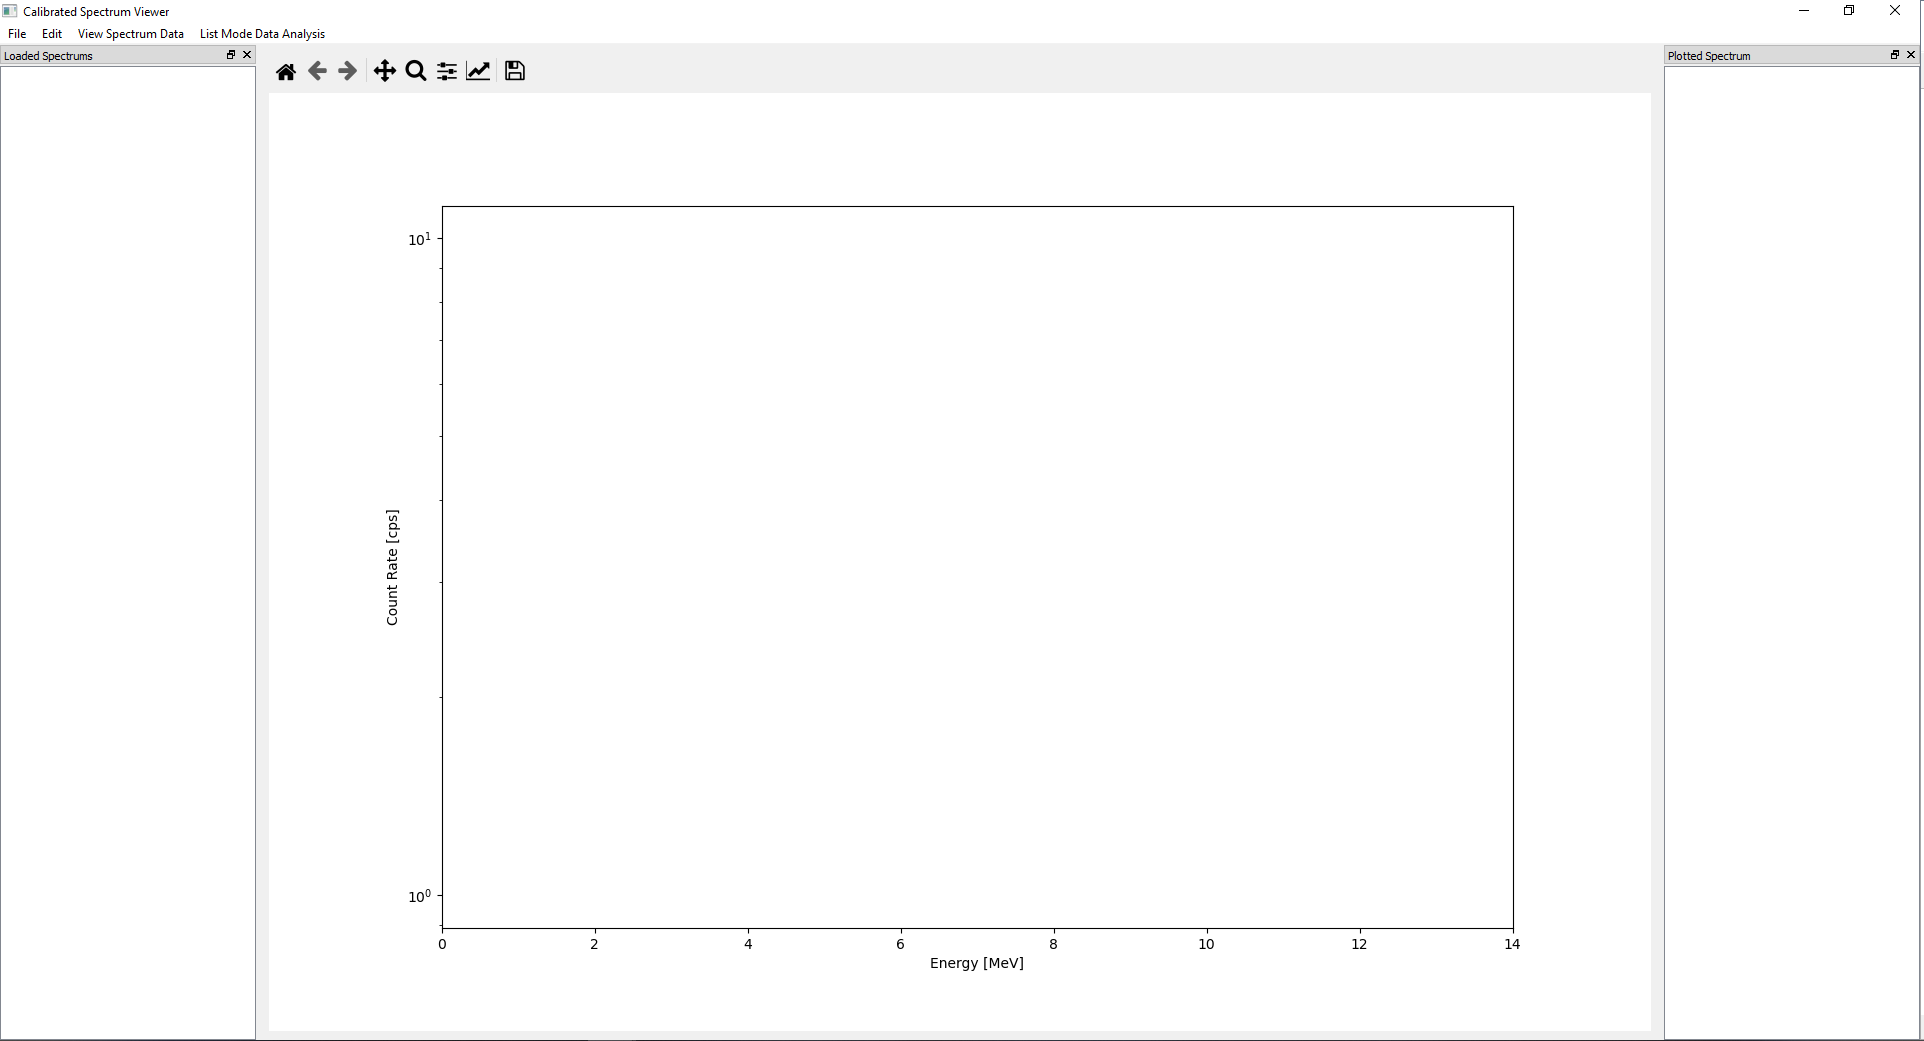
\includegraphics[width=\linewidth]{Front_Panel.png}
	\caption{User interface upon initial startup.}
	\label{fig:opening}
\end{figure}

\section{Discussion of Graph Setup}
The graph is initiated to be a energy calibrated, count rate spectrum. The count rate by default is shown in logarithmic scale to reveal small magnitude peaks. The energy by default ranges from 0 to 14MeV, the should encompass to vast majority of all possible energies normally seen, this can be adjusted, but more about that in a later section. 

